\chapter{Architettura del Sistema}\label{chap:second}

\inlineminitoc

In questo capitolo viene presentata l'architettura complessiva del sistema sviluppato, illustrando i componenti principali e il flusso di dati attraverso le diverse fasi del processo. L'obiettivo è fornire una panoramica chiara e dettagliata delle scelte progettuali adottate per affrontare le sfide tecniche del progetto.

\section{Componenti del sistema}
I componenti sono presentati in ordine logico, rappresentando il percorso che i dati seguono dal momento in cui vengono acquisiti fino alla fase di interrogazione e utilizzo da parte degli utenti finali.

\begin{enumerate}
    \item \textbf{Estrazione dei Documenti:} Descrizione delle tecniche utilizzate per l'estrazione dei testi dai documenti normativi, con particolare attenzione alle strategie e alle librerie impiegate per il parsing e la pulizia dei dati.
    
    \item \textbf{Strutturazione dei Documenti:} Spiegazione del ruolo dei LLM nella trasformazione del testo estratto in un formato strutturato, con particolare attenzione alla definizione dello schema JSON utilizzato per rappresentare la gerarchia dei documenti normativi.
    
    \item \textbf{Archiviazione nei Database:} Descrizione delle tecnologie di storage utilizzate, con focus sui due principali database impiegati:
    \begin{enumerate}
        \item[3.1] \textbf{Database a Grafo \textit{(Neo4j)}:} Illustrazione della struttura del database e del processo di inserimento dei dati, con particolare attenzione alla modellazione delle informazioni e alla rappresentazione delle relazioni gerarchiche dei documenti normativi.
        \item[3.2] \textbf{Database Vettoriale \textit{(Qdrant)}:} Descrizione del processo di inserimento dei dati strutturati nel database
    \end{enumerate}
    
    \item \textbf{Implementazione della Ricerca Semantica:} Spiegazione dell'approccio adottato per la ricerca semantica, compresa la scelta dei modelli di embedding e le definizioni delle metriche di valutazione.
    
    \item \textbf{Benchmarking e Confronto tra Database:} Processo di benchmark condotto per valutare le prestazioni di ricerca, analizzando le differenze e le performance tra l'approccio basato su database a grafo e quello basato su database vettoriale.
\end{enumerate}
La figura \ref{fig:architettura-software} fornisce un diagramma riassuntivo dell'architettura del sistema, evidenziando i componenti principali e il flusso di dati tra di essi.

\begin{figure}[H]
    \centering
    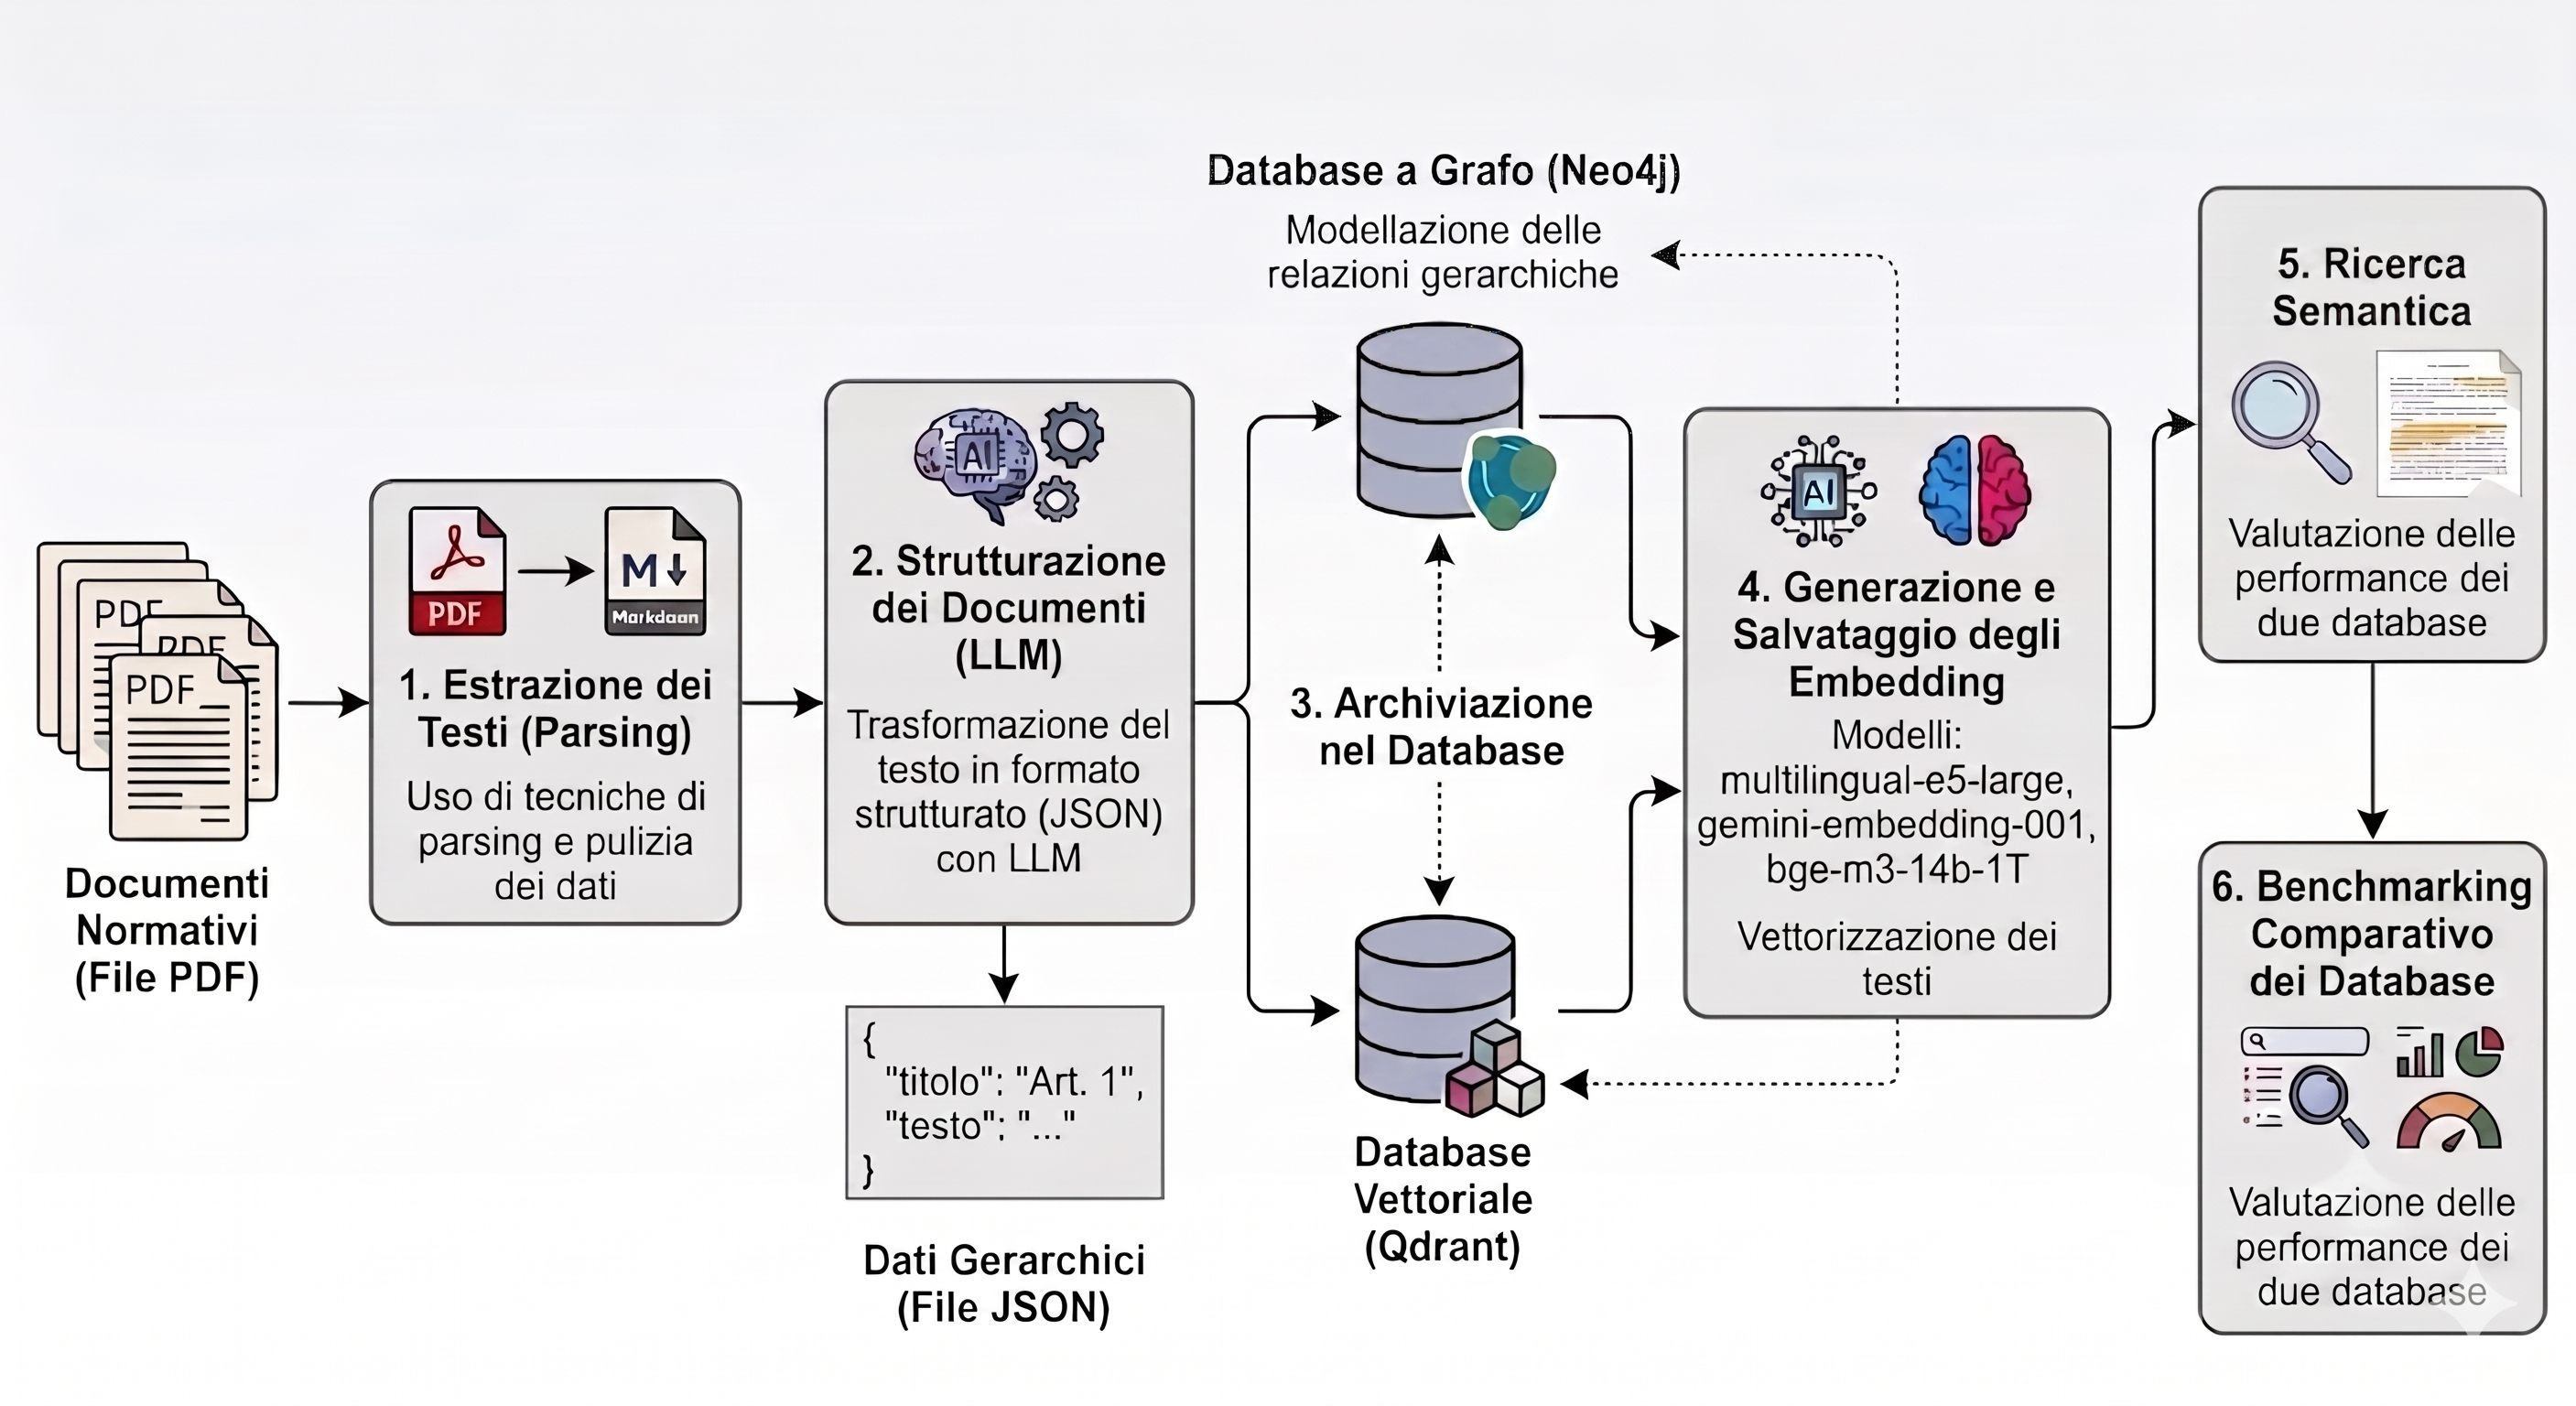
\includegraphics[width=1\textwidth]{_images/architettura-software.png}
    \caption{Architettura del sistema}
    \label{fig:architettura-software}
\end{figure}